% !TEX root = diss.tex

\chapter{The Relationship Between Arrhenius Pre-factors with Non-Covalent Binding}
\label{ch:arrhenius}

\section{Introduction}

DiLabio and Ingold\cite{DiLabio2005} previously investigated the formal HAT
reaction of the iminoxyl/oxime self-exchange reaction. In that paper, they
compiled a table of parameters from the phenomenological Arrhenius equation for
a series of interesting reactions, which appear here
in~\ref{tab:Arrhenius-expt}.\cite{Kreilick1966, Mader2004, Mahoney1970,
DaRooge1967, Howard1973, Foti1994, Chenier1974, Chenier1975} These are
thermoneutral hydrogen atom self-exchange reactions involving oxygen-centered
radicals, and other nearly thermoneutral reactions involving the destruction and
formation of oxygen-centered radicals, reactions 3.1 and 3.2, respectively:

\begin{align}
  \ch{$\pi$-RO^. + ROH &-> ROH + $\pi$-RO^.} \hspace{2cm} \Delta H = 0 \\
  \ch{$\pi$-R}^\prime\ch{O^. + ROH &-> R}^\prime\ch{OH + $\pi$-RO^.} \hspace{2cm} \Delta H \approx 0
\end{align}

\newcommand{\tabFig}[2][0.35]{\includegraphics[scale=#1]{figures/#2.eps}}

\begin{table}[!ht]
  \footnotesize
  \centering
  \caption[Table of results for (nearly) thermoneutral reactions
  studied.]{Table of results for (nearly) thermoneutral reactions studied. Units
  for $\Delta H$, $E_a$, and calculated pre-reaction complex binding energy (BE)
  are \kcalmol, $\log A$ are log \Ms, and $k$ are \Ms.\ References to the
  original literature are included with the Complex ID number.
  $^\dagger$Calculated binding energies involve structures that could not be
  fully optimized and contain one or more small imaginary frequencies. Adapted
  with permission from Reference \protect\citenum{DiLabio2005}. Copyright (2005)
  American Chemical Society.}
  \begin{tabular}{l >{\centering}m{1.5cm} >{\centering}m{1.5cm}
  >{\centering}m{1.2cm} >{\centering}m{1.2cm} >{\centering}m{1.2cm}
  >{\centering}m{1.2cm} >{\centering}m{0.8cm} m{0em}}
  ID & \ch{RO^.}/\ch{R}$^\prime$\ch{O^.} & \ch{ROH} & $\Delta H$ & $\log~A$ & $E_a$ & $k$ & BE & \\
  \toprule
  1\cite{Kreilick1966} & \tabFig{3tBuPhO} & \tabFig{3tBuPhOH} & 0.0 & 3.7 & 1.2 & 3.3\E{2} & -10.8 &\\
  2\cite{Mader2004} & \tabFig{4MeC5H4ONO} & \tabFig{4MeC5H6NOH} & -2.0 & 3.8 & 3.8 & 10 & -14.8 &\\
  3\cite{Kreilick1966}& \tabFig[0.4]{2tBuNO} & \tabFig[0.4]{2tBuNOH} & 0.0 & 5.1 & 3.5 & 3.3\E{2} & -10.1$^\dagger$ &\\
  4\cite{Mahoney1970,DaRooge1967} & \tabFig{3tBuPhO} & \tabFig{tBuPhOH} & 4.2 & 5.5 & 4.8 & 93 & -10.0$^\dagger$ &\\
  5\cite{Howard1973} & \tabFig[0.7]{tBuOO} & \tabFig{3tBuPhOH} & -7.0 & 4.2 & 0.5 & 7\E{3} & -6.5 &\\
  6\cite{Kreilick1966} & \tabFig[0.7]{Ph2NO} & \tabFig[0.7]{Ph2NOH} & 0.0 & $>$7 & - & $>$10$^7$ & -13.6$^\dagger$ &\\
  7\cite{Foti1994} & \tabFig{PhO} & \tabFig{2hydroxynaphthalene} & -2.2 & 8.3 & 2.3 & 4\E{6} & -8.6 &\\
  8\cite{Chenier1974} & \tabFig[0.7]{tBuOO} & \tabFig{PhOH} & 0.3 & 7.2 & 5.2 & 3\E{3} & -5.5$^\dagger$ &\\
  9\cite{Chenier1974} & \tabFig[0.7]{tBuOO} & \tabFig{2hydroxynaphthalene} & -1.9 & 6.4 & 2.6 & 3\E{4} & -5.6$^\dagger$ &\\
  10\cite{Chenier1975} & \tabFig[0.7]{tBuOO} & \tabFig{alphatetralinperoxide} & 1.4 & 6.0 & 4.5 & 7\E{2} & -8.0$^\dagger$ &
\end{tabular}
\label{tab:Arrhenius-expt}
\end{table}

Although it is well known that reactions of this nature involve remarkably low
activation energies ($E_a$),\cite{Lucarini1996, Mahoney1970a, Mahoney1975,
Korcek1972} the Arrhenius pre-exponential factors ($A$), or as they shall be
referred to herein, \emph{A-factors}, as a well as rate constants, span a wide
range (summarized in~\ref{tab:Arrhenius-expt}): The measured A-factors range
from $10^{3.5}$--$10^{8.3}$ \Ms\ and the rate constants range from 10--10\E{7}
\Ms.\ In the past, this range has been attributed to steric shielding around the
oxygen atoms, resulting in a larger entropic barriers.\cite{DiLabio2005}
Importantly, it was noted that the degree of steric shielding on the oxygen atom
appears to play an important role in the order of the A-factor; systems with
greater bulk have lower A-factors, while non-shielded systems have larger
A-factors.

Stereo-electronic effects are known to play an important role in HAT, and have
been studied extensively.\cite{Finn2004, Salamone2011, Pischel2001, Griller1981,
Bietti2011, Salamone2012, Malatesta1982, Salamone2014} Although the abstraction
of a specific hydrogen atom may be more thermodynamically favourable than others
on a given substrate, if it is not accessible due to steric constraints,
abstraction will not occur at this site. Otherwise, additional steric bulk can
lead to significant reductions in reactivity, through destabilization of the TS
complex, or by forcing additional processes involving conformational changes in
order to reach the appropriate TS structure. For example, in reactions of
tertiary acetamides with \cumo,\cite{Salamone2014} where abstraction occurs
mainly from C-H bonds $\alpha$ to the nitrogen atom, a two-fold decrease in the
rate constant (normalized for the number of equivalent hydrogen atoms) is
observed in going from $N,N$-dimethylacetamide to $N,N$-diisobutylacetamide
($k_H$ = $2.0 \times 10^5$ and $7.8 \times 10^4$ \Ms, respectively). The
decrease in rate constant is attributed to the steric clash between the methyl
groups of \cumo\ and the isobutyl groups of $N,N$-diisobutylacetamide.

As all of the reactions in~\ref{tab:Arrhenius-expt} are nearly thermoneutral,
thermochemical effects on the rates of reaction are expected to be minimal.
Therefore, the large degree of variance in their rate constants ($k$) is
somewhat surprising. These reactions are closely related to the self-exchange
reaction between phenol and phenoxyl,\cite{Mayer2002} in which a strong
molecule-radical pre-reaction complex akin to those listed
in~\ref{tab:Arrhenius-expt} is formed, ca. 10 \kcalmol\ below the separated
reactants. It is therefore expected that most, if not all, of the systems
in~\ref{tab:Arrhenius-expt} should exhibit a similar molecule-radical complex;
granted, the strength of the interaction will vary because of steric repulsion.
As such, it is plausible that the strength of this interaction may directly
influence the rate of formal hydrogen atom transfer.

Currently, there has been no comprehensive investigation of the relationship
between the pre-reaction complex and the kinetics of a reaction. On the basis of
the reaction data in~\ref{tab:Arrhenius-expt}, we ask the question: \emph{Do
A-factors have a correlation with non-covalent binding energies of the
pre-reaction complex?} This is a reasonable question as non-covalent binding and
steric hinderance represent a loss of degrees of freedom and therefore
entropy,\footnotemark\ which ultimately determines the A-factor magnitude. If
the answer to the question is yes, then non-covalent binding may be useful as a
diagnostic for the ``looseness'' or ``tightness'' of a TS complex, in addition
to providing an important link between theory and experiment.

\footnotetext{Recall from Equation~\ref{eq:afactor} that the A-factor can be
related to TST such that the primary variable is entropy ($\Delta^\ddagger
S^0$).}


\section{Computational methods and details}

Density-functional theory (DFT) calculations were carried out using the
Gaussian-09 software package.\cite{Frisch2009} Care was taken to obtain minimum
energy structures through detailed conformational analysis. For this, the BLYP
density-functional\cite{Becke1988,Lee1988} was utilized, paired with the
empirical D3 dispersion correction\cite{Grimme2010} with the recommended
Becke-Johnson damping functions,\cite{Johnson2006} as well as our groups' own
basis set incompletion potentials (BSIPs),\cite{OterodelaRoza2017ACP} and
minimal MINIs basis sets.\cite{Huzinaga1984} The use of minimal basis sets
corrected for basis set incompleteness allows DFT-based methods to be used
efficiently in performing a large number of calculations. Minimum energy
conformers of the monomers (substrates and radicals) were first obtained by
manual manipulation of the necessary dihedral bond angles, followed by geometry
optimization and vibrational analysis.

The lowest energy radicals and substrates were combined to generate the
appropriate pre-reaction complexes. These pre-reaction complexes were subject to
conformational analysis using the same BLYP-D3(BJ)-BSIP/MINIs method. Geometries
were initially manipulated by hand. It became apparent that manual manipulation
resulted in an unsatisfactory exploration of the conformational space. To solve
this, all the necessary dihedral angles were scanned systematically using a
combination of scripts.\bibnote{The Escher program
(https://github.com/aoterodelaroza/escher) was used to
generate a Z-matrix with specific dihedral angles. This geometry was then
systematically scanned using simple shell scripts.} All manipulated geometries
were subject to optimization. For each complex, the top 5--10 complex geometries
were subject to further optimization using a higher level of theory
(BLYP-D3(BJ)-BSIP/pc-1) to obtain the final minimum energy pre-reaction complex
structures. Due to the free rotation of groups such as $t$-butyl and methyl,
some of the optimized pre-reaction complex structures contain small imaginary
frequencies, and thus do not represent proper stationary states. Several
measures were taken to resolve this, however, no resolution was obtained in many
cases. Regardless, the complexes adequately represent the pre-reaction complex
and differences in ``true'' binding energies can likely be ignored.

To obtain accurate pre-reaction complex binding energies, the substrates and
complexes were subject to single-point energy calculations using the
LC-$\omega$PBE long-range corrected density functional\cite{Vydrov2006,
Vydrov2006a} with D3(BJ) dispersion corrections and pc-2 basis sets with
$f$-type basis functions removed (pc-2-spd).\cite{Johnson2013} This method was
selected on the recommendation of work by \citet{Johnson2013}, which
demonstrated the accuracy of this method for the calculation of NCIs. On the
basis of the reported mean absolute error in Reference \citenum{Johnson2013} for
the S66 benchmark set of sixty-six different non-covalently interacting
dimers,\cite{Rezac2011} the calculated binding energies reported herein from the
LC-$\omega$PBE-D3(BJ)/pc-2-spd level of theory carry an estimated 0.2 \kcalmol\
margin of error.

\section{Results and discussion}

The theoretically determined electronic binding energies calculated for the
lowest energy pre-reaction complex of each system are listed
in~\ref{tab:Arrhenius-expt}. The logarithm of A-factor against binding energy
was plotted, as shown in~\ref{fig:Arrhenius}. The overall correlation is quite
poor ($R^2$ = 0.33), however much of the data is grouped about a single, well
correlated line ($R^2$ = 0.95). The intercept of the fitted line that
corresponds to zero binding energy is 8.63, a value that is in line with what
has been cited as the expected A-factor for HAT reactions, \emph{viz.
}$10^{8.5\pm0.5}$ \Ms.\cite{Benson1976} These results suggest that the observed
correlation is genuine, that is, NCIs may have an impact on A-factors. I shall
demonstrate that the data that do not correlate are reasonable outliers. In
fact, using simple rationale I shall demonstrate that different regimes of
steric bulk results in different mechanistic processes leading to the TS
complex.

\begin{figure}[!htbp]
  \centering
  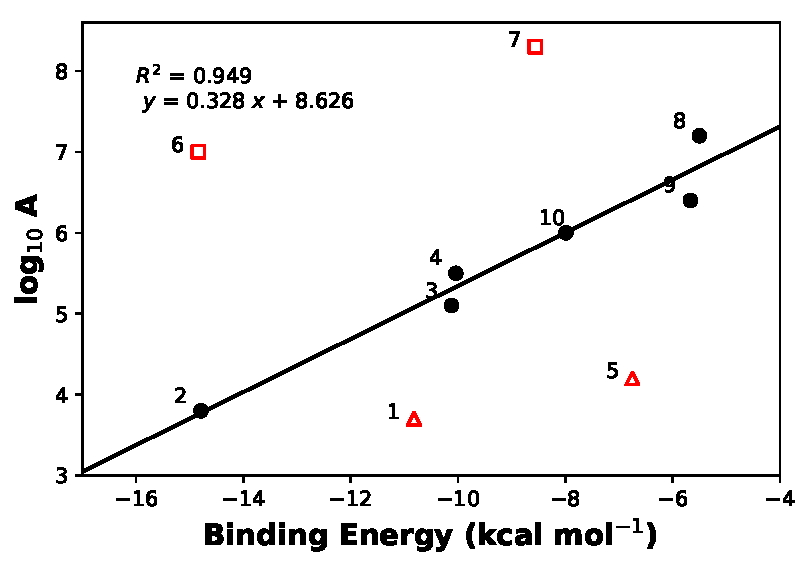
\includegraphics[width=0.85\textwidth]{figures/arrhenius-scatter.pdf}
  \caption[Plot of logarithm of A-factor against binding energy.]{Plot of
  logarithm of A-factor against binding energy. Only the black points were
  included in the line fitting (slope = 0.328 \kcalmol, intercept = 8.626
  \kcalmol, and $R^2$ = 0.949). Red points with open faced markers indicate
  outliers, \emph{vide infra}. The inclusion of complexes 1, 5, and 7 result in
  an $R^2$=0.334. Complex 6 is always omitted from line fitting as the
  experimental A-factor is approximate.}
  \label{fig:Arrhenius}
\end{figure}

In order to understand the deviations from the expected linear trend of A-factor
against pre-reaction complex binding energies, it is important to consider the
specific reaction mechanisms taking place. Recall from Chapter~\ref{ch:intro}
that we are focussed on two important possible reaction mechanisms, namely
direct HAT and PCET.

For direct HAT to occur, the SOMO of the radical must overlap with the O-H
$\sigma^*$ anti-bonding orbital. In the case of hydrogen abstraction from a
phenolic compound, this may require the rotation of the hydrogen atom donating
hydroxyl group out of the plane. The rotation of a phenolic hydroxyl group has
an energy barrier that follows a $\cos^2 \theta$ relationship.\cite{Kojima1960}
As a reference point, the rotational barrier of phenol\cite{Kim1994} is 3.1
\kcalmol, thus sterically hindered phenols may have a greater rotational
barrier. For a PCET mechanism to occur, there are two possible geometries:
The nominally singly-occupied O $2p$-orbital of the radical overlaps can
overlap with the corresponding oxygen LP $2p$-orbital, as seen in the work of
\citet{Mayer2002}. Alternatively, a LP-$\pi$, LP-LP, or $\pi$-$\pi$ bonding
overlap between the radical and substrate can occur, as seen in the work of
\citet{DiLabio2005}, and \citet{DiLabio2007}.

As described in Chapter~\ref{ch:intro}, there remains no clear physical criteria
to distinguish direct HAT from PCET, a topic that remains of active the
literature.\cite{Cukier1998, Mayer2002, Stubbe2003, Mayer2004, DiLabio2007,
Huynh2007, HammesSchiffer2008, Mayer2010, Weinberg2012, HammesSchiffer2015,
MunozRugeles2017} One possible solution is consider the existence of these
mechanisms exists on a continuum; the rate constant (and thus A-factor) for
formal HAT ($k_{HAT}$) can be described as a combination of the rate constants
direct HAT ($k_{direct}$) and PCET ($k_{PCET}$) mechanisms, i.e.:

\begin{equation}
  k_{HAT} = k_{direct} + k_{PCET}
  \label{eq:A-theory}
\end{equation}

Before elaborating on Equation~\ref{eq:A-theory}, we must first discuss the role
of the pre-reaction complexes in formal HAT reactions. As a radical and
substrate approach sufficient proximity for a reaction to take place, NCIs lead
to the formation of a weakly bound complex. If this complex has the appropriate
geometry for a hydrogen transfer to occur, it is considered a pre-reaction
complex, otherwise it is considered an initial encounter complex. An initial
encounter complex must pass over an additional energy barrier to reach the
appropriate pre-reaction complex. With respect to the species
in~\ref{tab:Arrhenius-expt}, the complexes formed involve various degrees of
$\pi$-$\pi$, LP-$\pi$, and LP-LP interactions, which contribute to the weakly
attractive, dispersion interactions. Furthermore, these same orbital
interactions in the TS complex can lead to the formation of an additional
electronic channel, enabling a PCET mechanism.\cite{DiLabio2005, DiLabio2007}
Returning now to Equation~\ref{eq:A-theory}, the different types of orbital
interactions may control the contributions of $k_{PCET}$ to the overall rate
constants.

While the data herein explore only the geometries of the pre-reaction complexes
involved in the hydrogen transfer reactions, the presumptive TS structures will
have similar structures and more importantly, orbital interactions. Therefore,
by considering the similarities between pre-reaction and TS complexes, it is
possible to rationalize the deviations from the observed trendline
in~\ref{fig:Arrhenius}.

\begin{figure}[!htbp]
  \centering
  \hspace*{-1.8cm}
  \begin{minipage}{8cm}
    \centering
    \begin{overpic}[width=\textwidth]{figures/complex2_hbond}
    \put(5,89) {\large\textbf{A.}}
  \end{overpic}
  \end{minipage}%
  \begin{minipage}{8cm}
    \centering
    \begin{overpic}[width=\textwidth]{figures/complex3_hbond}
    \put(5,90) {\large\textbf{B.}}
  \end{overpic}
  \end{minipage}
  \caption[Three-dimensional structures of pre-reaction complexes 2 (TEMPO-H and
  4-oxo-TEMPO) and 3 (di-$t$-butyl-hydroxylamine and
  di-$t$-butyl-nitroxyl).]{Three-dimensional structures of \textbf{A} complex 2
  (TEMPO-H and 4-oxo-TEMPO) and \textbf{B} complex 3 (di-$t$-butyl-hydroxylamine
  and di-$t$-butyl-nitroxyl). Bond distances are shown in units of \AA.\@ The
  elements are coloured as white for carbon, light blue for hydrogen, red for
  oxygen, and blue for nitrogen.}
  \label{fig:com2-3}
\end{figure}

I shall begin by examining the points that fall on the expected line, complexes
2--4 and 8--10. The examination of all these pre-reaction complexes reveals that
an additional rearrangement that has a moderate energetic barrier is required in
order for the hydrogen transfer to proceed. Complexes 2 and 3 are shown
in~\ref{fig:com2-3}, and are very similar in structure. Both are
hydroxylamine-nitroxyl couples with similar degrees of steric bulk adjacent to
the reacting centres. The $t$-butyl groups of 3, and the methyl groups of 2 (the
NO-ON dihedral angles are 65$^\circ$ and 68$^\circ$, respectively) prevent the
overlap of the N LP orbitals in of the NO-H-ON frameworks to allow for PCET.
Thus, while the presumptive TS structure may have some degree of LP-LP orbital
interaction, the overall mechanism is dominated by direct HAT.

In the most stable stacked conformation, complex 4, as seen in~\ref{fig:com4},
steric clash of the para-position $t$-butyl groups obstructs $\pi$-$\pi$ overlap
between the aromatic rings. It is likely that this steric clash does not allow
any significant orbital interaction, suggesting that the reaction is dominated
by direct HAT. In order to react via direct HAT, the hydroxyl group must rotate
further out of the aromatic plane, or the bulky para-position $t$-butyl groups
must come into close proximity. Alternatively, an open conformation for complex
4 is possible, which lies ca. 2 \kcalmol\ higher in energy than the stacked
complex, a result that is also consistent with the observed trend-line. From
the open conformation, PCET is still not possible due to the steric bulk of the
ortho-position $t$-butyl groups of the radical, thus this reaction likely also
proceeds through a direct HAT mechanism.

\begin{figure}[!htbp]
  \centering
  \hspace*{-1.8cm}
  \begin{minipage}{8cm}
    \centering
    \begin{overpic}[width=\textwidth]{figures/complex4_hbond}
    \put(10,107) {\large\textbf{A.}}
  \end{overpic}
  \end{minipage}%
  \begin{minipage}{8cm}
    \centering
    \begin{overpic}[width=\textwidth]{figures/complex4_steric}
    \put(0,105) {\large\textbf{B.}}
  \end{overpic}
  \end{minipage}
  \caption[Three-dimensional structure of pre-reaction complex 4 between
  2,4,6-tri-$t$-butylphenol and  4-$t$-butylphenoxyl.]{Three-dimensional
  structure of pre-reaction complex 4 between 2,4,6-tri-$t$-butylphenol and
  4-$t$-butylphenoxyl. \textbf{A} demonstrates the hydrogen bond distances in
  units of \AA, and the out-of-plane rotation by 35.2$^\circ$ of the phenolic
  hydroxyl group. \textbf{B} demonstrates the steric clash (highlighted by red
  box) between the para-position $t$-butyl groups. The elements are coloured as
  white for carbon, light blue for hydrogen, and red for oxygen.}
  \label{fig:com4}
\end{figure}

Complexes 8 and 9 are similar systems, in which \ch{$t$-BuOO^.} reacts with
unhindered phenolic substrates. As seen by the structures in~\ref{fig:com8-9},
the bound complexes are somewhat dissimilar. The hydroxyl group of complex 8 is
rotated out of the plane 24$^\circ$, while in complex 9 the hydroxyl group lies
entirely in the plane. It is likely that the larger aromatic system of
2-naphthol results in a larger OH rotational barrier, and thus the most
favourable conformation is entirely in the plane. In complex 9, there is also a
weak hydrogen bond between the C-H bond in the ortho-position and the
non-radical O-centre of \ch{$t$-BuOO^.}, contributing further to the
stabilization of the planar conformation. Complex 8 was previously studied by
\citet{DiLabio2007}, where it was demonstrated that a partial bonding
interaction exists between the peroxyl LP and phenolic $\pi$-system in the TS
complex. However, this interaction is likely weak thus contributes weakly to the
overall rate constant.  That is, $k_{HAT}$ is dominated by $k_{direct}$. Also,
although the pre-reaction complexes are somewhat dissimilar, the conformational
changes necessary to reach the TS complex, similar to that reported in reference
\citenum{DiLabio2007}, are likely not dramatically different in terms of
energetic barriers. Any small differences result in noise in the observed trend.

\begin{figure}[!htbp]
  \centering
  \hspace*{-1.8cm}
  \begin{minipage}{8cm}
    \centering
    \begin{overpic}[width=\textwidth]{figures/complex8_hbond}
    \put(5,102) {\large\textbf{A.}}
  \end{overpic}
  \end{minipage}%
  \begin{minipage}{8cm}
    \centering
    \begin{overpic}[width=\textwidth]{figures/complex9_hbond}
    \put(0,100) {\large\textbf{B.}}
  \end{overpic}
  \end{minipage}
  \caption[Three-dimensional structures of pre-reaction complexes 8
  ($t$-butylperoxyl and phenol) and 9 ($t$-butylperoxyl and
  2-naphthol).]{Three-dimensional structures of pre-reaction \textbf{A} complex
  8 ($t$-butylperoxyl and phenol) and \textbf{B} complex 9 ($t$-butylperoxyl and
  2-naphthol). Bond distances are shown in units of \AA.\@ Complex 8 has an out
  of plane rotation of the phenolic hydroxyl group of 24.1$^\circ$. The elements
  are coloured as white for carbon, light blue for hydrogen, and red for
  oxygen.}
  \label{fig:com8-9}
\end{figure}

Complex 10, shown in~\ref{fig:com10} is unique in that it is the only reaction
between a peroxide and a peroxyl radical. Therefore, this system represents the
best case scenario for LP-LP overlap to occur. The self-exchange reaction
between \ch{HOO^.} and \ch{HOOH} can be considered the simplest reference for
the reaction of $\alpha$-tetralin peroxide with $t$-butylperoxyl. To the best of
my knowledge, the mechanism of the hydroperoxyl-hydrogen peroxide couple has not
been characterized as either PCET or direct HAT previously in the literature,
although the TS structure has been previously reported.\cite{Isborn2005} Using
this structure, calculations reveal a LP-LP interaction leading to partial
bonding in the TS, i.e.\ a PCET mechanism. (See
Appendix~\ref{ap:arrhenius},~\ref{fig:hooh-ooh}). The hydroperoxyl-hydrogen
peroxide couple contains a \ch{H-O-O-H} dihedral angle of 90$^\circ$, so that
the two non-reacting hydrogen atoms oriented 180$^\circ$ away from one another.
Orienting substituents directly away from one another is likely the most stable
TS structure for all peroxyl-peroxide formal HAT reactions.

Complex 10 is unlikely to orient $t$-butylperoxyl and $\alpha$-tetralin peroxide
exactly 180$^\circ$ away from one another  due to steric clash. Nonetheless,
there may still be some LP-LP overlap contributing to a weak $k_{PCET}$
contribution to $k_{HAT}$. On the basis of the line fit in~\ref{fig:Arrhenius},
and given that the other point are dominated by $k_{direct}$, the same is likely
true in the case of complex 10. This means that either the TS structure does not
allow for sufficient LP-LP overlap for $k_{PCET}$ to dominate, or LP-LP overlap
does not allow for a strong PCET contribution to $k_{HAT}$. This will require
additional investigation.

\begin{figure}[!htbp]
  \centering
  \hspace*{-1.8cm}
  \begin{minipage}{8cm}
    \centering
    \begin{overpic}[width=\textwidth]{figures/complex10_hbond}
    \put(0,102) {\large\textbf{A.}}
  \end{overpic}
  \end{minipage}%
  \begin{minipage}{8cm}
    \centering
    \begin{overpic}[width=\textwidth]{figures/complex10_steric}
    \put(0,100) {\large\textbf{B.}}
  \end{overpic}
  \end{minipage}
  \caption[Three-dimensional structure of pre-reaction complex 10 between
  $t$-butylperoxyl and $\alpha$-tetralin peroxide.]{Three-dimensional structure
  of pre-reaction complex 10 between $t$-butylperoxyl and $\alpha$-tetralin
  peroxide. \textbf{A} demonstrates the hydrogen bond distances in units of \AA.
  \textbf{B} demonstrates the likely steric clash preventing strong LP-LP
  overlap. The elements are coloured as white for carbon, light blue for
  hydrogen, and red for oxygen.}
  \label{fig:com10}
\end{figure}

Once again, complexes 2--4 and 8--10 follow the observed trend. In all cases,
these complexes may have some PCET contribution to $k_{HAT}$ through either
LP-$\pi$ or LP-LP orbital overlap. Interpretation of~\ref{fig:Arrhenius} in this
manner allows for two possible explanations. The simplest is that all these
complexes proceed through a mechanism in which $k_{HAT} \approx k_{direct}$
($k_{PCET} \ll k_{direct}$). In this case, the A-factor is a direct reflection
of $k_{HAT}$ and this the pre-reaction complex binding energy correlates well
with the A-factor.

Alternatively, there may be increasing contributions of PCET leading to an
increase in the A-factor. This effect can be rationalized on the basis of a
stronger interaction in the case of LP-$\pi$ overlap, as compared to LP-LP
overlap. Within this framework, complexes 2, 3, and 4 may have little or no
overlap due to steric clashing, and complexes 8 and 9 have a higher A-factor
than complex 10 due to LP-$\pi$ vs. LP-LP overlap. Further work is necessary to
discern this effect.

Consider next the points that sit above the trendline, complexes 6 and 7, shown
in~\ref{fig:com6} and~\ref{fig:com7}. The A-factor for complex 6 is approximate
and thus does not get factored into the line fitting. In both cases, the
non-covalently bound complexes are in a slipped-parallel $\pi$-stacked
conformation, allowing for $\pi$-$\pi$ orbital overlap.  Complex 7 in particular
is very similar to the phenol-phenoxyl couple, except with 2-naphthol instead of
phenol. In both cases, the $\pi$-stacked pre-reaction complex is very close to
the presumptive TS structure. Therefore, it is possible to infer that both of
these reactions take place through mechanism in which $k_{PCET}$ is dominant.
The key difference from the points that fall on the trendline is that $k_{HAT}
\approx k_{PCET}$.

\begin{figure}[!htbp]
  \centering
  \hspace*{-1.8cm}
  \begin{minipage}{8cm}
    \centering
    \begin{overpic}[width=\textwidth]{figures/complex6_hbond}
    \put(5,90) {\large\textbf{A.}}
  \end{overpic}
  \end{minipage}%
  \begin{minipage}{8cm}
    \centering
    \begin{overpic}[width=\textwidth]{figures/complex6_pipi}
    \put(0,100) {\large\textbf{B.}}
  \end{overpic}
  \end{minipage}
  \caption[Three-dimensional structure of pre-reaction complex 6 between
  $N,N$-diphenylhydroxylamine and $N,N$-diphenylnitroxyl.]{Three-dimensional
  structures of pre-reaction complex 6 between $N,N$-diphenylhydroxylamine and
  $N,N$-diphenylnitroxyl. \textbf{A} demonstrates the hydrogen bonding
  interaction while \textbf{B} demonstrates the $\pi$-$\pi$ interaction.
  Distances in unit of \AA\ and angles are shown in degrees. The elements are
  coloured as white for carbon, light blue for hydrogen, blue for nitrogen, and
  red for oxygen.}
  \label{fig:com6}
\end{figure}

\begin{figure}[!htbp]
  \centering
  \hspace*{-1.8cm}
  \begin{minipage}{8cm}
    \centering
    \begin{overpic}[width=\textwidth]{figures/complex7_hbond}
    \put(0,80) {\large\textbf{A.}}
  \end{overpic}
  \end{minipage}%
  \begin{minipage}{8cm}
    \centering
    \begin{overpic}[width=\textwidth]{figures/complex7_pipi}
    \put(0,78) {\large\textbf{B.}}
  \end{overpic}
  \end{minipage}
  \caption[Three-dimensional structure of pre-reaction complex 7 between
  2-naphthol and phenoxyl.]{Three-dimensional structures of pre-reaction complex
  7 between 2-naphthol and phenoxyl. \textbf{A} demonstrates the hydrogen
  bonding interaction while \textbf{B} demonstrates the $\pi$-$\pi$ interaction.
  Distances in unit of \AA\ and angles are shown in degrees. The elements are
  coloured as white for carbon, light blue for hydrogen, and red for oxygen.}
  \label{fig:com7}
\end{figure}

Lastly, consider the points that fall below the trendline, complexes 1 and 5. In
both cases, a high degree of steric repulsion likely does not allow for a PCET
mechanism through orbital overlap. It is important to study the ``encounter
complex'' that represents the first pre-reaction complex, i.e. prior to any
reorganization, as this will be the complex that affects the A-factor with
regards to simple collision theory. Complex 1 is the self-exchange reaction
between the very bulky 2,4,6-tri-$t$-butylphenol/2,4,6-tri-$t$-butylphenoxyl
couple, as seen in~\ref{fig:com1-5} A. As a result of steric shielding around
the reaction centres, the encounter complex is stacked to maximize dispersion
interactions, but does not have a hydrogen bond. Therefore, an additional
rearrangement is required in order to get to the presumptive TS structure. That
is, there must be a higher-energy hydrogen-bonded pre-reaction couple that leads
to the direct HAT mechanism. Note however, that there is a barrier to rotation
of the hydroxyl group to 90$^\circ$ out of the plane for direct HAT to occur.

\begin{figure}[!htbp]
  \centering
  \hspace*{-1.8cm}
  \begin{minipage}{8cm}
    \centering
    \begin{overpic}[width=\textwidth]{figures/complex1}
    \put(0,93) {\large\textbf{A.}}
  \end{overpic}
  \end{minipage}%
  \begin{minipage}{8cm}
    \centering
    \begin{overpic}[width=\textwidth]{figures/complex5_new}
    \put(0,95) {\large\textbf{B.}}
  \end{overpic}
  \end{minipage}
  \caption[Three-dimensional structures of pre-reaction complexes 1
  (2,4,6-tri-$t$-butylphenoxl and 2,4,6-tri-$t$-butylphenoxyl) and 5
  (2,4,6-tri-$t$-butylphenol and $t$-butylperoxyl).]{Three-dimensional
  structures of pre-reaction \textbf{A} complex 1 (2,4,6-tri-$t$-butylphenoxl
  and 2,4,6-tri-$t$-butylphenoxyl) and \textbf{B} complex 5
  (2,4,6-tri-$t$-butylphenol and $t$-butylperoxyl). Distances in unit of \AA\
  and angles are shown in degrees. The elements are coloured as white for
  carbon, light blue for hydrogen, and red for oxygen.}
  \label{fig:com1-5}
\end{figure}

Complex 5 is the 2,4,6-tri-$t$-butylphenol/$t$-butylperoxyl reaction couple. The
encounter pre-reaction complex also does not contain a hydrogen bond. As with
complex 1, an encounter complex without a hydrogen bond must form
first. However, in complex 5 there is less steric clashing. As a result the
formation of a hydrogen bond is favourable and the ``true'' pre-reaction complex
is about 0.7 \kcalmol\ more stable than the encounter complex. In contrast, for
complex 1 the true pre-reaction complex is about 0.6 \kcalmol\ less stable than
the encounter complex. Note also that there is a barrier to
rotation\footnotemark\ of the hydroxyl group that can be estimated as about 4.1
\kcalmol. This is illustrated schematically in~\ref{fig:encounter-pes}.

\footnotetext{Calculated as the difference in energy between the in-plane and
out-of-plane structures of 2,4,6-tri-$t$-butylphenol at the
LC-$\omega$PBE-D3/6-311+G(2d,2p) level of theory.}

\begin{figure}[!htbp]
  \centering
  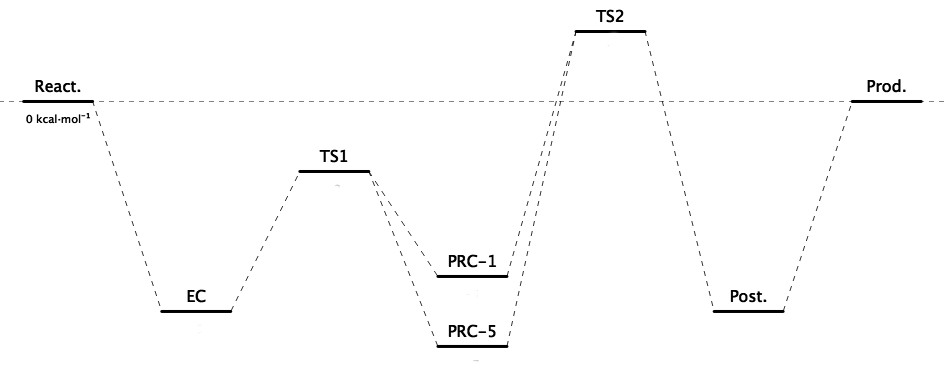
\includegraphics[width=\textwidth]{figures/encounter-pes.png}
  \caption[Reaction coordinate illustrating proposed mechanism for HAT in
  complexes 1 and 5.]{Reaction coordinate illustrating proposed mechanism for
  HAT in complexes 1 and 5. React. = reactants, EC = encounter complex,
  PRC-1/5. = true pre-reaction complex 1/5, TS1 = transition state associated
  with out-of-plane rotation of the OH group, TS2 = (presumptive) TS associated
  with HAT, Post. = post-reaction complex, Prod. = products.}
  \label{fig:encounter-pes}
\end{figure}

For both complex 1 and 5, steric clashing prevents significant $\pi$-$\pi$
overlap or LP-$\pi$ overlap. Therefore, the reactions likely proceed through a
direct HAT dominated mechanism ($k_{HAT} \approx k_{direct}$). One might then
expect these data to fall on the trendline, however the formation of an
encounter complex that does not lead directly to HAT results in a different
overall process from the other complexes. As a result of the necessary initial
process complex 1 and 5 have lower A-factors as less collisions are likely to
lead to successful formal HAT.


\section{Summary}

In this investigation, a series of thermoneutral or nearly thermoneutral HAT
reactions were considered. I have plotted the theoretically determined
electronic binding energies against the logarithm of experimentally determined
A-factors. These results demonstrate that the A-factors for (nearly)
thermoneutral HAT reactions correlate to some extent with the pre-reaction
complex binding energies, given that the reactions proceed through similar
mechanisms and energetically similar pathways. The results herein can be sorted
into three bins by considering the contributions of $k_{direct}$ and $k_{PCET}$
to the overall transformation, $k_{HAT}$:

\begin{enumerate}
  \item Complexes that have weak $k_{PCET}$ contributions due to either LP-LP
	  or LP-$\pi$ orbital overlap, and are therefore dominated by
	  $k_{direct}$. This is the case for the data that fall on the
	  trendline.

  \item Complexes in which $k_{PCET}$ is the dominant contribution to
	  $k_{HAT}$, as is the case for complexes 6 and 7.

  \item Complexes in which the encounter complex does not lead directly the
  HAT TS complex, as was the case for complexes 1 and 5.
\end{enumerate}

These results indicate that different regimes of electronic and steric
interactions lead to different chemical processes in seemingly similar
reactions. As a results, non-covalent binding can be used as a metric for
kinetics parameters, however, it cannot describe in full the entropic factors
that contribute to the A-factor. One must first consider the mechanistic
details in which formal HAT occurs.

Additional work is necessary to extend these results. In particular, the main
question that remains is whether $\pi$-$\pi$ PCET is ``better'' than other
forms of orbital overlap. To answer this a larger sample of data points, and a
diagnostic for PCET must be used. Regardless, the results herein represent a
novel attempt to link theory and experiment. Given that obtaining the full PES
for large molecules is currently computationally impractical, these results
serve as a seed for developing a fundamental understanding of complex formal HAT
reactions.
